
\def\theTopic{Helper--Hinderer }
\def\dayNum{4}


\begin{center}
\vspace*{-.2in}
{\bf {\large Helper -- Hinderer}}\\
\end{center}

Do young children know the difference between helpful and unhelpful
behavior?  You read about a study in   {\it Nature}\footnote{ Hamlin, J. K.,
  Wynn, K., \& Bloom, P. (2007). Social evaluation by preverbal
  infants. {\it Nature}, 450, 557-559. } which
reported results from a simple study of infants which was intended to
check young kids' feelings about helpful and non-helpful behavior.  
  The research question is:
\begin{center}
  {\sf Are infants able to notice and react to helpful or hindering
    behavior observed in others?} 
\end{center}

{\bf Data}:  Of the 16 infants age 6 to 10 months, 14 chose the ``helper'' toy
and 2 chose the ``hinderer''.

{\bf Discuss with your group and fill in:	}\vspace{-.3cm}
\begin{enumerate}
  \item  What proportion of the infants chose the helper toy? Include
    the correct notation. ($p$ for a population proportion, or
    $\phat$ for the sample proportion.)
\begin{students}
     \vspace{1cm}
\end{students}

\begin{key}
     {\it  $\phat = 14/16 = 0.875$ }
\end{key}
\item  
     Suppose the infants really had no preference for one toy or the other,
     and the puppet show had no effect.  What sort of results
     (numbers) would     you expect to see?
\begin{students}
       \vspace{1cm}
\end{students}

\begin{key}
       {\it  Close to 1/2 picking the helper.}
\end{key}

   \item Think back to our ``Martian Alphabet'' activity on the first day of
     class.  What sort of evidence made us think that humans could
     decipher Martian script?  Note:  it depended not just on how many
     people in the class got it right, but also on 
     the ``background'' distribution from the coin flips or the spinner.
\begin{students}
  \vspace{2cm}
\end{students}

\begin{key}
       {\it   We saw that relative to the spinner, the the class got
         an unusually high number correct.}
\end{key}
 
   \item How could you use coin flips to model a child's choice of
     toy? For 16 kids?
\begin{students}
  \vspace{2cm}
\end{students}

\begin{key}
       {\it  For one kid, let Heads = ``Helper'', tails =
         ``Hinderer''.  Count the proportion of heads in 16 flips of a
         fair coin.} 
\end{key}
   \item In using the coin, what assumption are you making about the
     kids' preferences? 
\begin{students}
  \vspace*{2cm}
\end{students}

\begin{key}
       {\it   That they are just picking one toy at random with no
         real preference for the helper or hinderer.}
\end{key}

   \item In statistical language the idea of ``no preference'' is
     called the {\bf null hypothesis}  and it is written in terms of
     the population proportion, $p=$ the true proportion of infants
     who chose the helper toy, as
      $$ H_0:\ p = 0.5.$$
     We also have an {\bf alternative hypothesis}, labeled $H_a$,
     which tells us the direction the researchers would like to
     conclude is true.  For this situation, they think there might be
     a preference toward the helper, so they would like to conclude
     that $H_0$ is wrong, and that really 
       $$H_a: \ p > 0.5 \mbox{ is true.}$$

     Under $H_0$,  is it possible that 14 out of 16
      infants could have chosen the helper toy just by chance? 
\begin{students}
  \vspace{1cm}
\end{students}

\begin{key}
{\it Yes, it is possible to get 14 or more heads. Anything is
  possible in a random sequence, but it is not very likely. }
\end{key}

\item If infants had no real preference, would the observed result (14
  of 16 choosing the helper) be very surprising or somewhat
  surprising, or not so surprising? How strong do you believe the
  evidence is against the null hypothesis?
\begin{students}
  \vspace{2cm}
\end{students}

\begin{key}
{\it Pretty surprising, strong evidence against the null.}
\end{key}

%% Use a spinner here?

  \item         {\bf Carry Out the Simulation}\\
     To see that happen, use the
     \url{https://jimrc.shinyapps.io/Sp-IntRoStats}  web app. Under
     the \fbox{One Categ} menu select \fbox{Spinner}.  Set the  
        Number of categories to \fbox{2}, Labels to \fbox{help, hinder},
        Percentages to \fbox{50,50}, Stop after \fbox{Fixed number of
          spins}, Last spin: \fbox{16}, and click \fbox{Run} to
        see a simulation of 16 kids choosing helper or hinderer when
        the two are equally likely. Record the number of ``helpers'',
        click \fbox{Run} again, and write down that number as well.
\begin{students}
  \vspace{1.5cm}
\end{students}

\begin{key}
{\it 12 in my first, 8 in my second }
\end{key}

    \item  Set  \fbox{1000} or more trials,  \fbox{Run}, and   
              sketch your plot of 1000 trial results. 
\begin{students}
  \vspace{4cm}
\end{students}

\begin{key}
    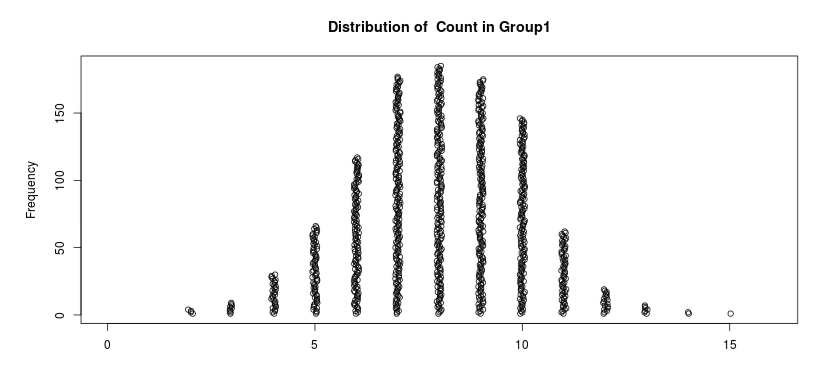
\includegraphics[width=.8\linewidth]{../plots/Helper16.png}
\end{key}
\item To see how unusual it is to get 14 or more ``helpers'' add the
  counts (for 14, 15, 16) in the table below the plot.
   How many of yours are this extreme? Circle
  these dots on your plot above. Check with the other groups
  nearby. Do we all agree?
\begin{students}
  \vspace{1.5cm}
\end{students}

\begin{key}
{\it  AWV, typically zero to 5.
}
\end{key}
\item  Do you think that babies are just randomly choosing one of
      the toys? Explain.
\begin{students}
  \vspace{1.5cm}
\end{students}

\begin{key}
  {\it No, because it is unlikely that the observed result will pop up
    if  kids are really picking at random. }
\end{key}

  \end{enumerate}
  You read about p-value or ``Strength of evidence'' in the reading
  for today.   To help interpret strength of evidence, we offer this picture:
 \begin{figure}[h]
   \centering
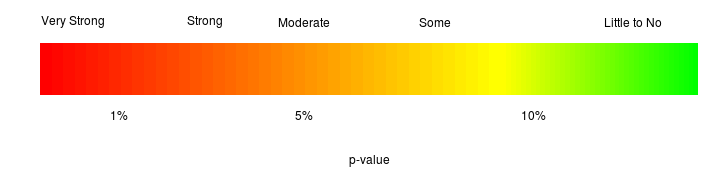
\includegraphics[width=\linewidth]{../plots/pvalueStrengths.png}
   \caption{Numeric p--value and strength of evidence}
   \label{fig:SOE-pvalue}
 \end{figure}

  The important point is that {\bf smaller} p--values (in red) provide {\bf
    stronger} evidence against $H_0$ and then $H_0$ gets a ``red
  light''. Red indicates that we don't believe it.  We will soon talk
  about actually rejecting $H_0$ when the evidence against it is
  strong.  Notation to watch:  strong evidence is always against the
  null. We never have strong evidence in favor of the null.  



\begin{enumerate}
  \setcounter{enumi}{11}

    \item  Use your plot from above to quantify the strength of
      evidence for the observed result 
      of 14 out of 16 infants choosing the helper toy. Give the
      numeric p--value  and a verbal description of the evidence it provides.
\begin{students}
  \vspace{1.5cm}
\end{students}

\begin{key}
{\it  1/1000 on my simulation which is ``Very Strong'' evidence
  against $H_0$.}
\end{key}

\item Explain in your own words why {\bf smaller} p-values provide
  {\bf stronger}   evidence against $H_0$.
\begin{students}
  \vspace{2cm}
\end{students}

\begin{key}
{\it AWV}
\end{key}

\item  What does this suggest about infants making their
      selections based only on random chance?
\begin{students}
  \vspace{2cm}
\end{students}

\begin{key}
{\it It suggests they do not make their choices based on random
 chance and do make decisions based on social interactions. }
\end{key}
\item Summarize how the p-value is computed.
\begin{students}
  \vspace{2cm}
\end{students}

\begin{key}
{\it By comparing the observed result to a distribution we get when
  $H_0$ is true. Take the points as or more extreme and divide by the
  number of points.}
\end{key}

\item  Put the following steps into their proper order:
 \begin{enumerate}
      \item  report strength of evidence 
\begin{key}
          {\it 5}
\end{key}
      \item  gather data 
\begin{key}
        {\it  2}
\end{key}

      \item  formulate a hypothesis 
\begin{key}
{\it 1   }
\end{key}


      \item  simulate a distribution 
\begin{key}
        {\it  3}
\end{key}
      \item  compare observed results to the distribution 
\begin{key}
        {\it  4}
\end{key}

  \end{enumerate}
\end{enumerate}

{\bf Take Home Messages}
\begin{itemize}
  \item Setting up null and alternative hypotheses is very
    important.\\
    They should be set in the planning stages of the study, not after
    looking at the data. 
    The equals sign always goes into $H_0$, but the value we set $ = p$ is not
    always .5.  The direction of the inequality in $H_a$ must match
    the researcher's ideas -- what they would like to show. It can be
    $<$, $>$, or $\neq$.  The latter means they are looking for a
    difference in either direction.
  \item It's important to know the definition of the p--value. We
    assume $H_0$ is true to compute it.  We  use a simulation based
    on the  value for $p$  in $H_0$ to calculate the p--value.    
  \item The idea of p--value is very important in statistics. It will
    follow us all the way through the course. Stronger evidence means
    {\bf smaller} p--value.  Large p--values mean the data are not
    unusual under $H_0$.
  \item In any hypothesis test, we report p--values to the reader.  
\end{itemize}\vfill

{\bf Assignment}
\begin{itemize}
\item   D2Quiz 2 on D2L by 11 pm Jan 25.
\item  {\bf D2Box 2} is due Jan 28.  Turn in as a pdf file to the D2L
  drop box.
\item The last page of this course pack  is a review table. You should
  tear it out and fill it in as we go. You will be able to bring it
  with you to exams.  You can now fill in the top five boxes  in column 1.
\item Read the next two pages before the next class.
\item Watch video \#  5 on randomization distributions and
  hypothesis testing before class.  Review \# 4 as well.
 \item 
  Make your own summary of the lesson. \\
  Thinking back about the most important ideas of this lesson help
  cement them in your head and help you avoid cramming right before
  the exam.  Writing them here will make studying much easier.   
\end{itemize}


